%%
%% This is file `tikzposter-template.tex',
%% generated with the docstrip utility.
%%
%% The original source files were:
%%
%% tikzposter.dtx  (with options: `tikzposter-template.tex')
%%
%% This is a generated file.
%%
%% Copyright (C) 2014 by Pascal Richter, Elena Botoeva, Richard Barnard, and Dirk Surmann
%%
%% This file may be distributed and/or modified under the
%% conditions of the LaTeX Project Public License, either
%% version 2.0 of this license or (at your option) any later
%% version. The latest version of this license is in:
%%
%% http://www.latex-project.org/lppl.txt
%%
%% and version 2.0 or later is part of all distributions of
%% LaTeX version 2013/12/01 or later.
%%


\documentclass{tikzposter} %Options for format can be included here

\usepackage{todonotes}

\usepackage[tikz]{bclogo}
\usepackage{lipsum}
\usepackage{amsmath}

\usepackage{booktabs}
\usepackage{longtable}
\usepackage[absolute]{textpos}
\usepackage[it]{subfigure}
\usepackage{graphicx}
\usepackage{cmbright}
%\usepackage[default]{cantarell}
%\usepackage{avant}
%\usepackage[math]{iwona}
\usepackage[math]{kurier}
\usepackage[T1]{fontenc}


%% add your packages here
\usepackage{hyperref}
% for random text
\usepackage{lipsum}
\usepackage[english]{babel}
\usepackage[pangram]{blindtext}

\colorlet{backgroundcolor}{blue!10}

 % Title, Author, Institute
\title{Kaggle Project Report}
% \author{Shaoni Wang$^1$, Gang Li$^2$}
\author{Huanhuan Ge}
% \institute{$^1$ Xi'an Shiyou University, China \\
% 	$^2$ Deakin University, Australia
% }
\institute{Qingdao University of Technology, China
}
%\titlegraphic{logos/tulip-logo.eps}

%Choose Layout
\usetheme{Wave}

%\definebackgroundstyle{samplebackgroundstyle}{
%\draw[inner sep=0pt, line width=0pt, color=red, fill=backgroundcolor!30!black]
%(bottomleft) rectangle (topright);
%}
%
%\colorlet{backgroundcolor}{blue!10}

\begin{document}


\colorlet{blocktitlebgcolor}{blue!23}

 % Title block with title, author, logo, etc.
\maketitle

\begin{columns}
 % FIRST column
\column{0.5}% Width set relative to text width

%%%%%%%%%% -------------------------------------------------------------------- %%%%%%%%%%
 %\block{Main Objectives}{
%  	      	\begin{enumerate}
%  	      	\item Formalise research problem by extending \emph{outlying aspects mining}
%  	      	\item Proposed \emph{GOAM} algorithm is to solve research problem
%  	      	\item Utilise pruning strategies to reduce time complexity
%  	      	\end{enumerate}
%%  	      \end{minipage}
%}
%%%%%%%%%% -------------------------------------------------------------------- %%%%%%%%%%


%%%%%%%%%% -------------------------------------------------------------------- %%%%%%%%%%
\block{Introduction}{
\begin{description}
  \item This is a prediction problem. The datasets includes 7,398 movies and various metadata from the Movie
  Database (TMDB).We need to predict the worldwide revenue for 4398 movies.The datasets' attributes are shown below.
\end{description}
\vspace{.5cm}

\begin{tabular}{ p{14cm}p{23cm}}
  \toprule
  Name     &        Attirbute   \\
  \midrule
  sales\_train.csv     &  id,belongs\_to\_collection,budget,genres,homepage, 
                          imdb\_id,original\_language,original\_title,overview,
                          popularity,poster\_path,production\_companies,
                          production\_countries,release\_date,runtime,
                          spoken\_languages,status,tagline,title,Keywords,
                          cast,crew,revenue \\

  test.csv              & id,belongs\_to\_collection,budget,genres,homepage, 
                          imdb\_id,original\_language,original\_title,overview,
                          popularity,poster\_path,production\_companies,
                          production\_countries,release\_date,runtime,
                          spoken\_languages,status,tagline,title,Keywords,
                          cast,crew \\

  sample\_submission.csv      &  id,revenue\\
   \bottomrule
\end{tabular}
}
%%%%%%%%%% -------------------------------------------------------------------- %%%%%%%%%%


%%%%%%%%%% -------------------------------------------------------------------- %%%%%%%%%%
\block{Data processing}{
\begin{itemize}
    \item
    Basic Information of Data
    \item
    Numerical features
    \item
    Remove missing value and NaN value
    \item
    Filter outliers  Data
    \item
    Process Genres
    \item
    Process Date

\end{itemize}


}
%%%%%%%%%% -------------------------------------------------------------------- %%%%%%%%%%


%%%%%%%%%% -------------------------------------------------------------------- %%%%%%%%%%

%\note{Note with default behavior}

%\note[targetoffsetx=12cm, targetoffsety=-1cm, angle=20, rotate=25]
%{Note \\ offset and rotated}

 % First column - second block


%%%%%%%%%% -------------------------------------------------------------------- %%%%%%%%%%
\block{Data Visualization}{
  	% We propose the \emph{GOAM} algorithm to solve the research problem of
    % \emph{Group Outlying Aspects Mining}.
  	% The \emph{GOAM} algorithm includes three major steps.
    Graph of budget, popularity and revenue.
%    1) Group Feature Extraction,
%    2) Outlying Degree Scoring, and
%    3) Outlying Aspects Identification.

\begin{center}    
    \begin{minipage}{0.45\linewidth}
    \centering
    \begin{tikzfigure}
      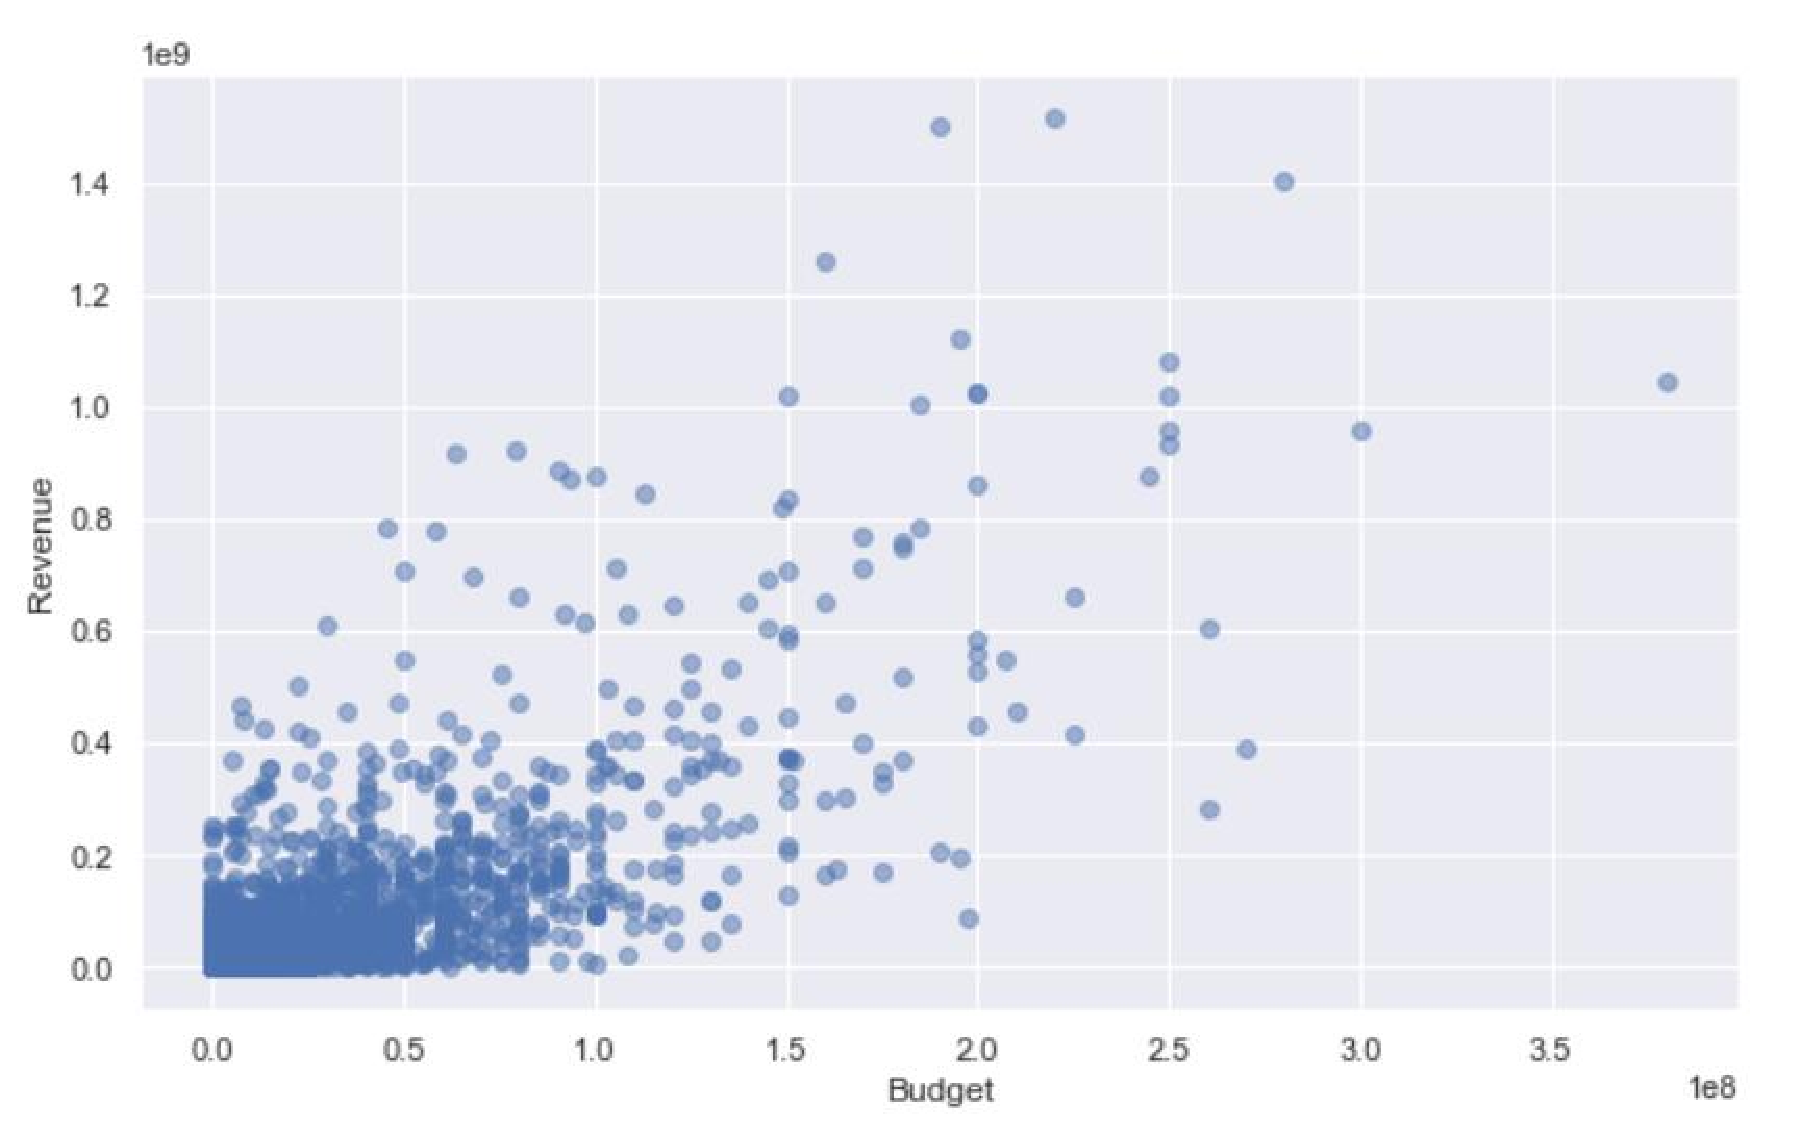
\includegraphics[width=0.9\linewidth]{figures/budget2.eps}
    \end{tikzfigure}%
    \end{minipage}
    \hfill
    \begin{minipage}{0.45\linewidth}
    \centering
    \begin{tikzfigure}
      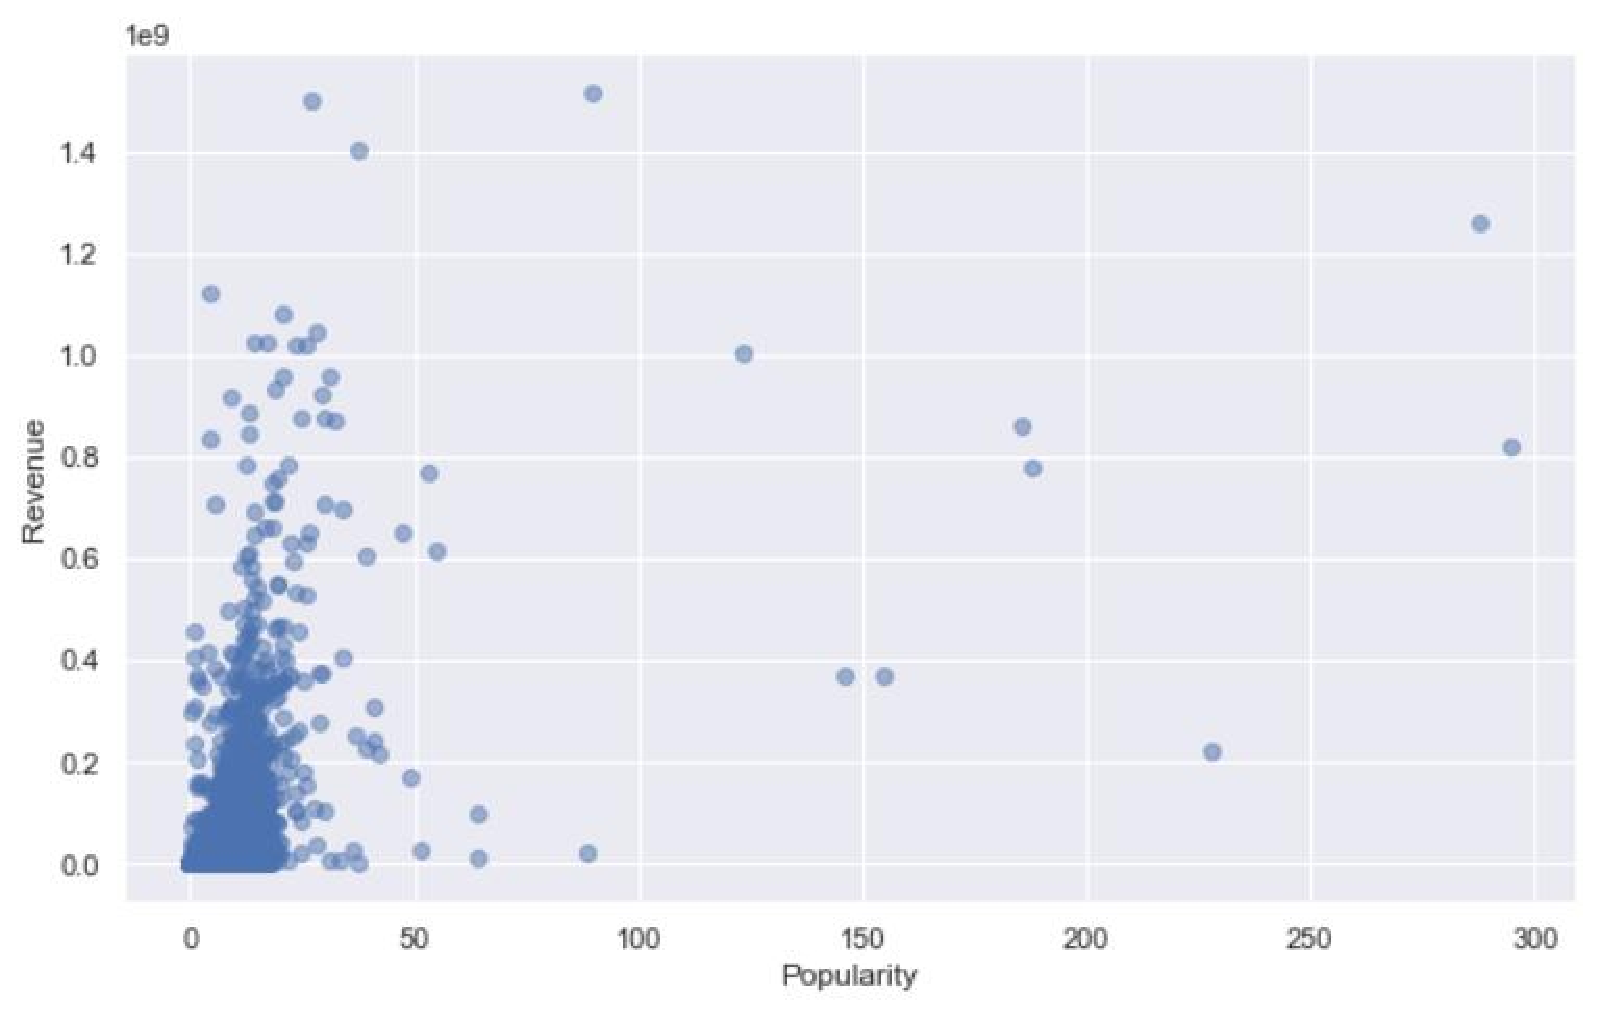
\includegraphics[width=0.9\linewidth]{figures/popular2.eps}
    \end{tikzfigure}%
    \end{minipage}
\end{center}

		
\begin{description}

    \item 
    Year And Revenue.

\end{description}
\begin{tikzfigure}
  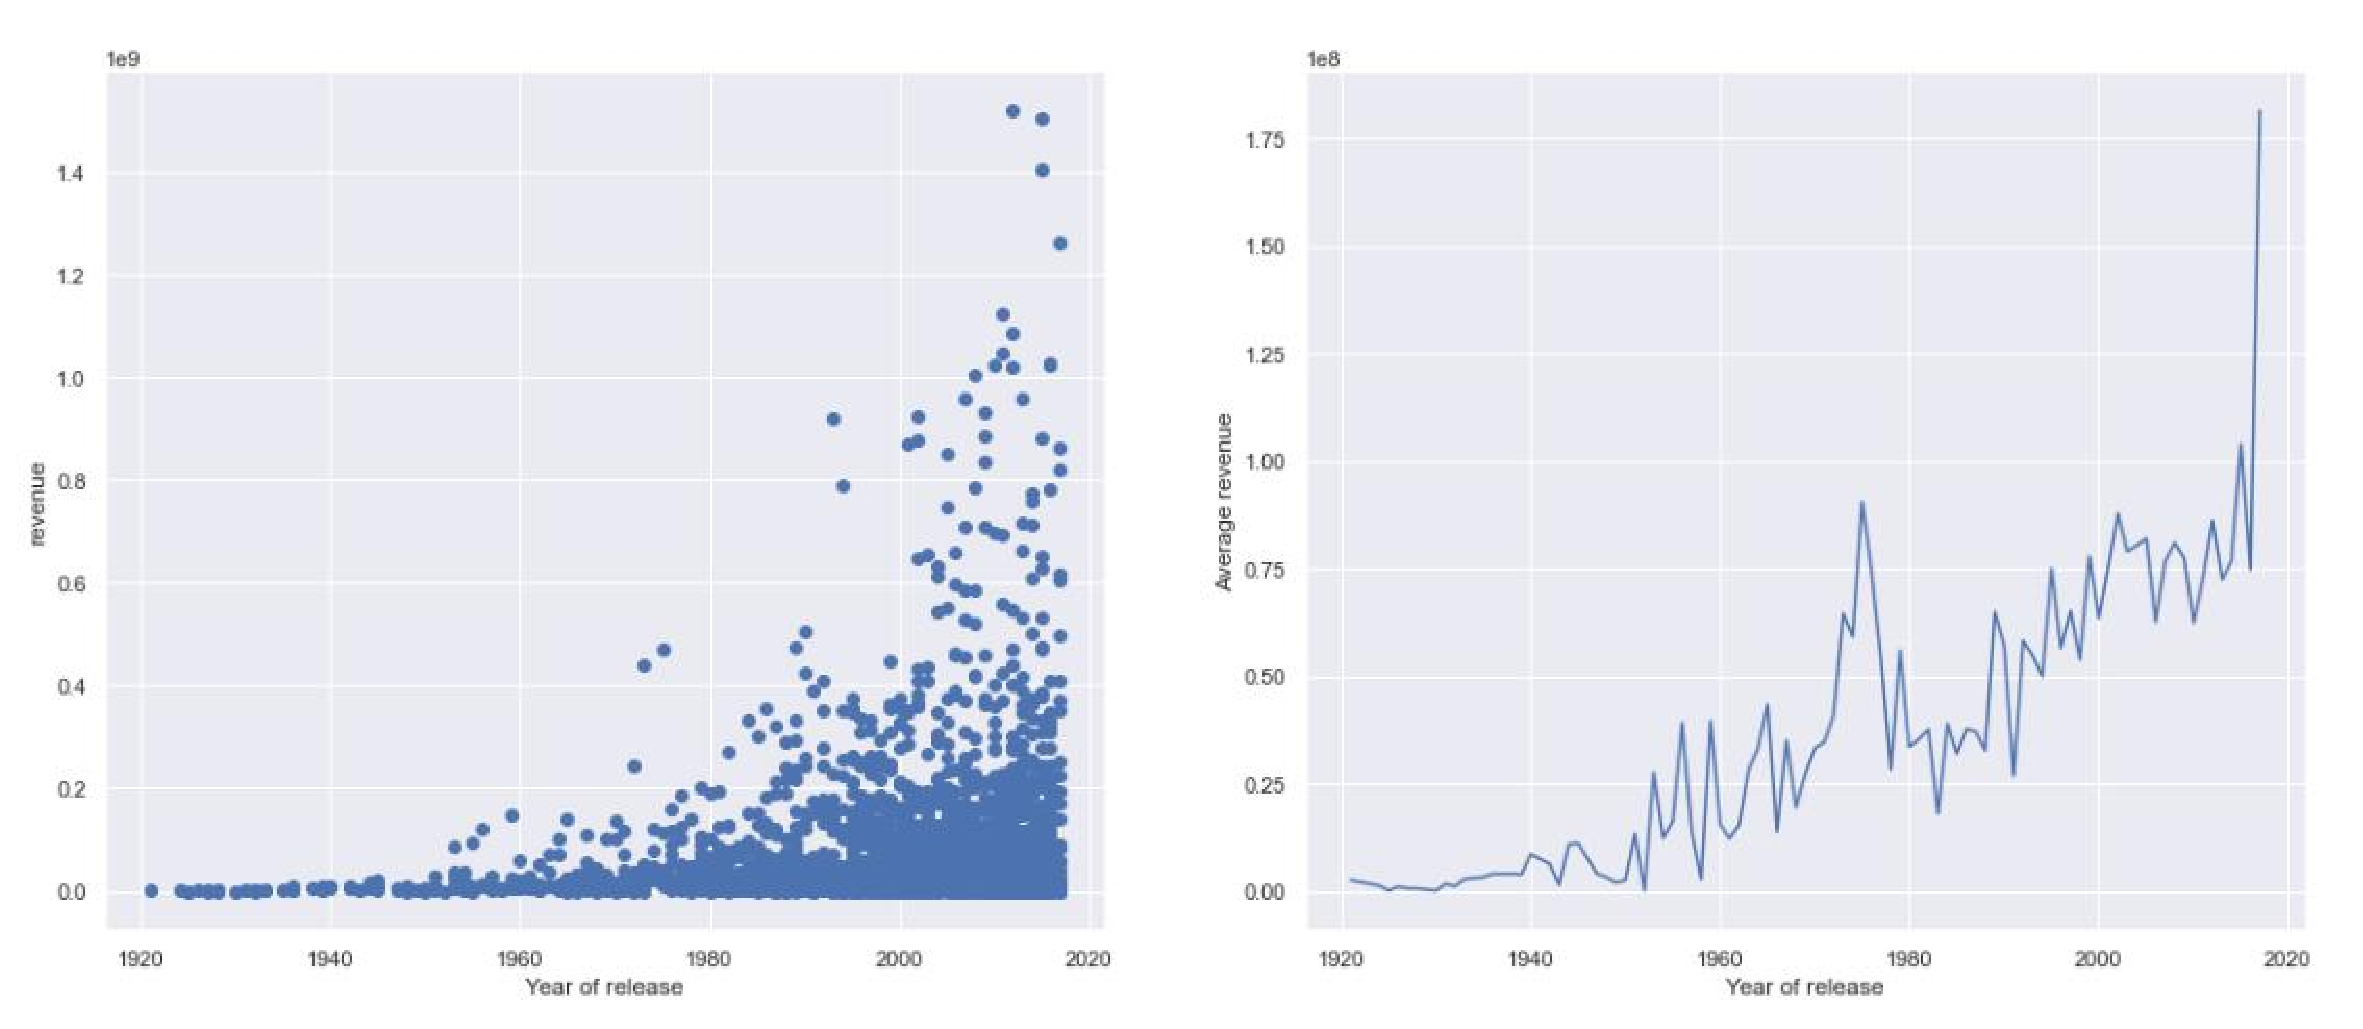
\includegraphics[width=0.8\linewidth]{figures/year2.eps}
 \end{tikzfigure}

}
%%%%%%%%%% -------------------------------------------------------------------- %%%%%%%%%%


% SECOND column
\column{0.5}
 %Second column with first block's top edge aligned with with previous column's top.

%%%%%%%%%% -------------------------------------------------------------------- %%%%%%%%%%
\block{Feature Selection}{
  \begin{itemize}
    \item
    release\_data: release\_year, release\_day, release\_month \\
    \item
    original\_language,number\_companies,crew\_size \\
    \item
    budget,popularity, runtime  \\
\end{itemize}
\begin{tikzfigure}
  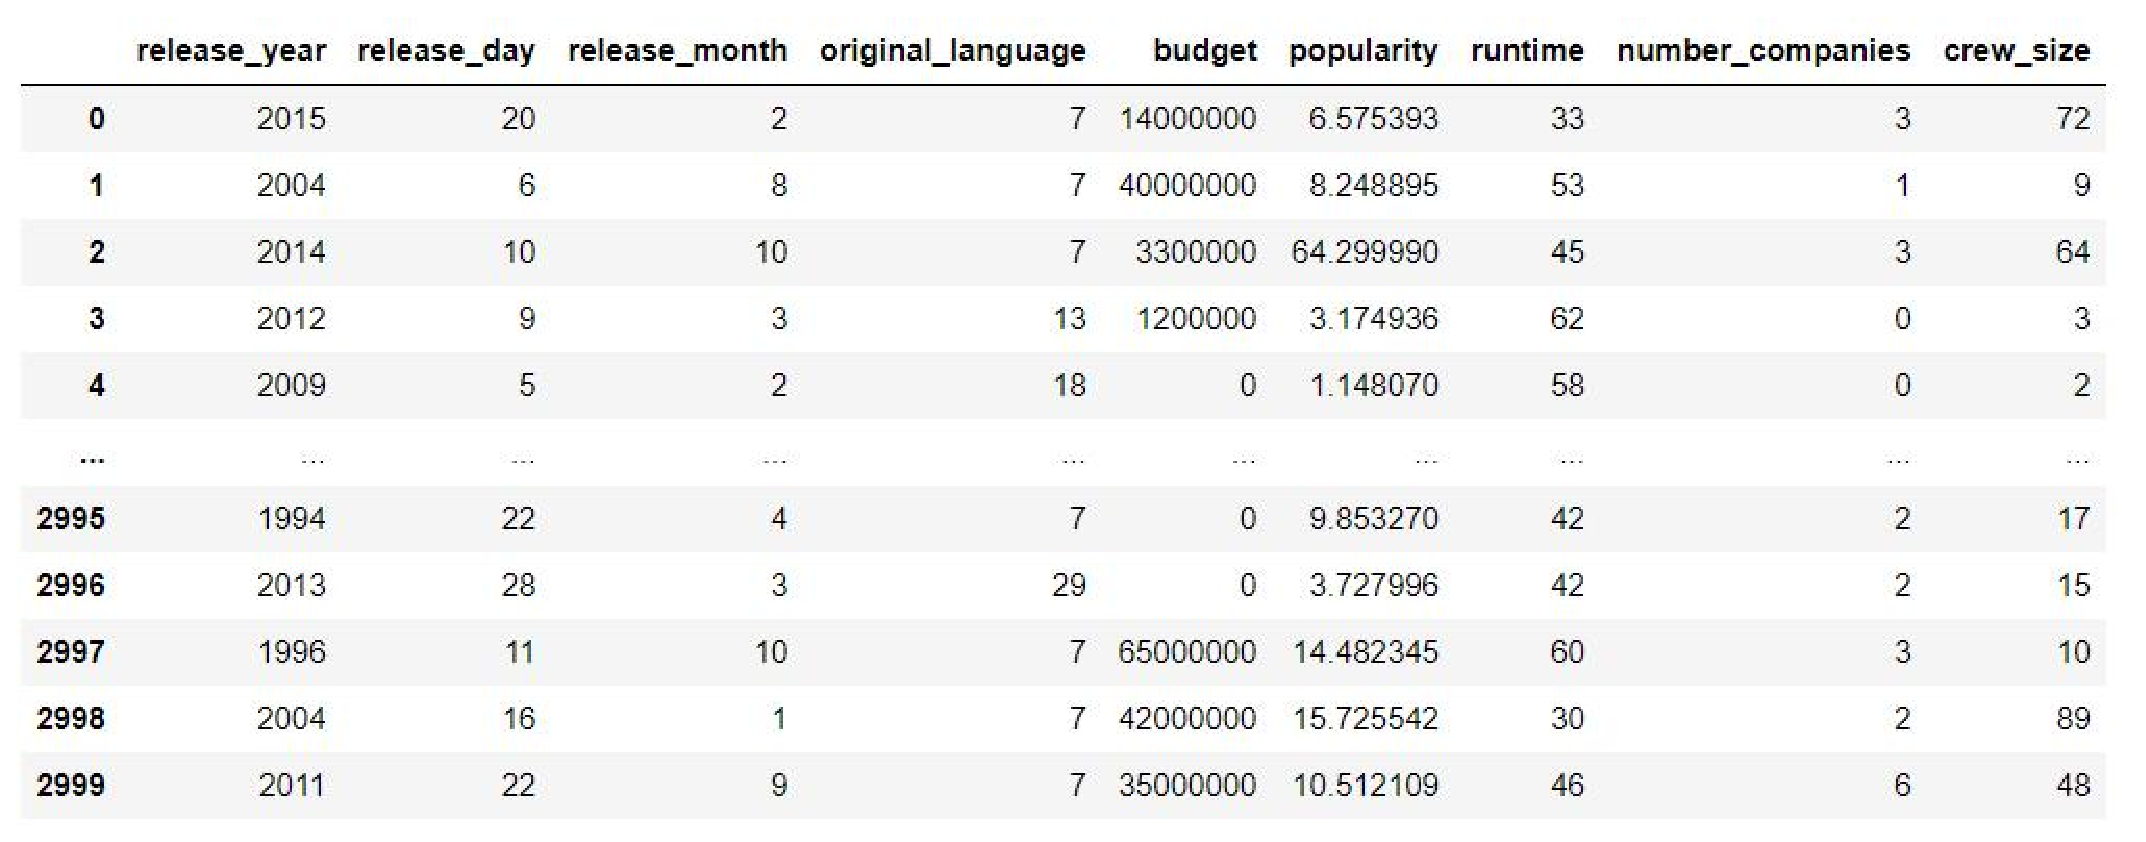
\includegraphics[width=0.9\linewidth,height=0.6\linewidth]{figures/feature1.eps}

 \end{tikzfigure}
}


%%%%%%%%%% -------------------------------------------------------------------- %%%%%%%%%%
\block[titleleft]{Modeling and Result}
{
  \begin{itemize}
    \item
    Model:Random Forest
    \begin{itemize}
      \item
      A random forest is a classifier that contains multiple decision trees and whose output class is
      determined by the plurality of the classes of the individual tree outputs.
    \end{itemize}
    \item
    RMSE
    \begin{itemize}
      \item
      The root mean square error is the square root of the ratio of the deviation between the predicted
      value and the true value to the number of observations n.
    \end{itemize}
    \item
    Train set: 0.8 , Test set: 0.2
    \item
    Score: 1.19
  \end{itemize}
}
%%%%%%%%%% -------------------------------------------------------------------- %%%%%%%%%%


% Second column - second block
%%%%%%%%%% -------------------------------------------------------------------- %%%%%%%%%%
\block[titlewidthscale=1, bodywidthscale=1]
{Conclusion}
{
\begin{description}
  \item
  The effect of the model is general, the main reason is that the selected features \\
   are not comprehensive enough, and the learning and thinking of feature  \\
   selection should be strengthened in the future. \\
\end{description}
}
%%%%%%%%%% -------------------------------------------------------------------- %%%%%%%%%%

\end{columns}


%%%%%%%%%% -------------------------------------------------------------------- %%%%%%%%%%
%[titleleft, titleoffsetx=2em, titleoffsety=1em, bodyoffsetx=2em,%
%roundedcorners=10, linewidth=0mm, titlewidthscale=0.7,%
%bodywidthscale=0.9, titlecenter]

%\colorlet{noteframecolor}{blue!20}
\colorlet{notebgcolor}{blue!20}
\colorlet{notefrcolor}{blue!20}
% \note[targetoffsetx=-13cm, targetoffsety=-12cm,rotate=0,angle=180,radius=8cm,width=.96\textwidth,innersep=.4cm]
\note[targetoffsetx=-13cm, targetoffsety=-15cm,rotate=0,angle=180,radius=8cm,width=.96\textwidth,innersep=.4cm]
{
\begin{minipage}{0.3\linewidth}
\centering
\includegraphics[width=24cm]{./graphics/logos/tulip-wordmark.eps}
\end{minipage}
\begin{minipage}{0.7\linewidth}
{ \centering
Kaggle Project Report,13/05/2022,qingdao,China
}
\end{minipage}
}
%%%%%%%%%% -------------------------------------------------------------------- %%%%%%%%%%


\end{document}

%\endinput
%%
%% End of file `tikzposter-template.tex'.